

\subsection{Short term abnormal returns in the Market Model} \label{ST_results}

With a baseline in the thesis' theoretical and methodological groundwork from prior sections, the following presents the main empirical results in relation to the hypotheses. 
To test hypothesis #1 of whether SDG-related events impacts firms' market values in the short term, I separate negative and positive events and assess the aggregated development in abnormal returns 10 days before and 10 days after an event has occurred. Moreover, I isolate the influence of individual SDGs to assess if events related to specific sustainability goals are more relevant for investors than other. The Market Model is applied to measure abnormal returns in all instances. For simplicity, when discussing negative events, I will mention the AAR as an absolute value. Thus, although the AAR decreases on the graph I will communicate the move as an increase in abnormal returns, since I assume we wish to take a short position in the assets. 

\subsubsection{Negative news} \label{sec: st_negative}

The average abnormal returns and development in cumulative average abnormal returns after a negative events are illustrated in figure \ref{fig:ST_neg_news}. To support the analysis, the 95\% confidence intervals of the AAR and CAAR are portrayed along with the amount of events on a given day relative to the event day $(t = 0)$ (right axis) illustrated by the white bars in the background. The left y-axis depicts the abnormal return and the x-axis is the number of days before and after an event has occurred. 

The average abnormal returns of the event date $(t=0)$ is significantly negative at -0.40\% at a 1\% level. Investors are reacting to spikes in bad news of firms by selling their shares. The days following an event demonstrates no abnormal performance. The abnormal returns are approximately zero on average until $t = -6$ upon which the AAR decreases in the days leading up to the event date, with the only significantly negative AARs found between $t=-6$ and $t=0$ at a $5\%$ level. Nonetheless, the CAAR is significantly negative from $t=-4$ and through the remaining window where it bottoms at approximately $-0.75\%$ 10 days after an event. The new information appears to be priced in prior to the spike in news articles. 

The declining nature of the CAAR suggests that the market gradually learns about the negative events upon which the prospective events are gradually priced in. After the spike in news on the event date the news has limited impact. \\ 


\begin{figure} [H]
    \centering
    \caption{Negative news: AAR and CAAR}
    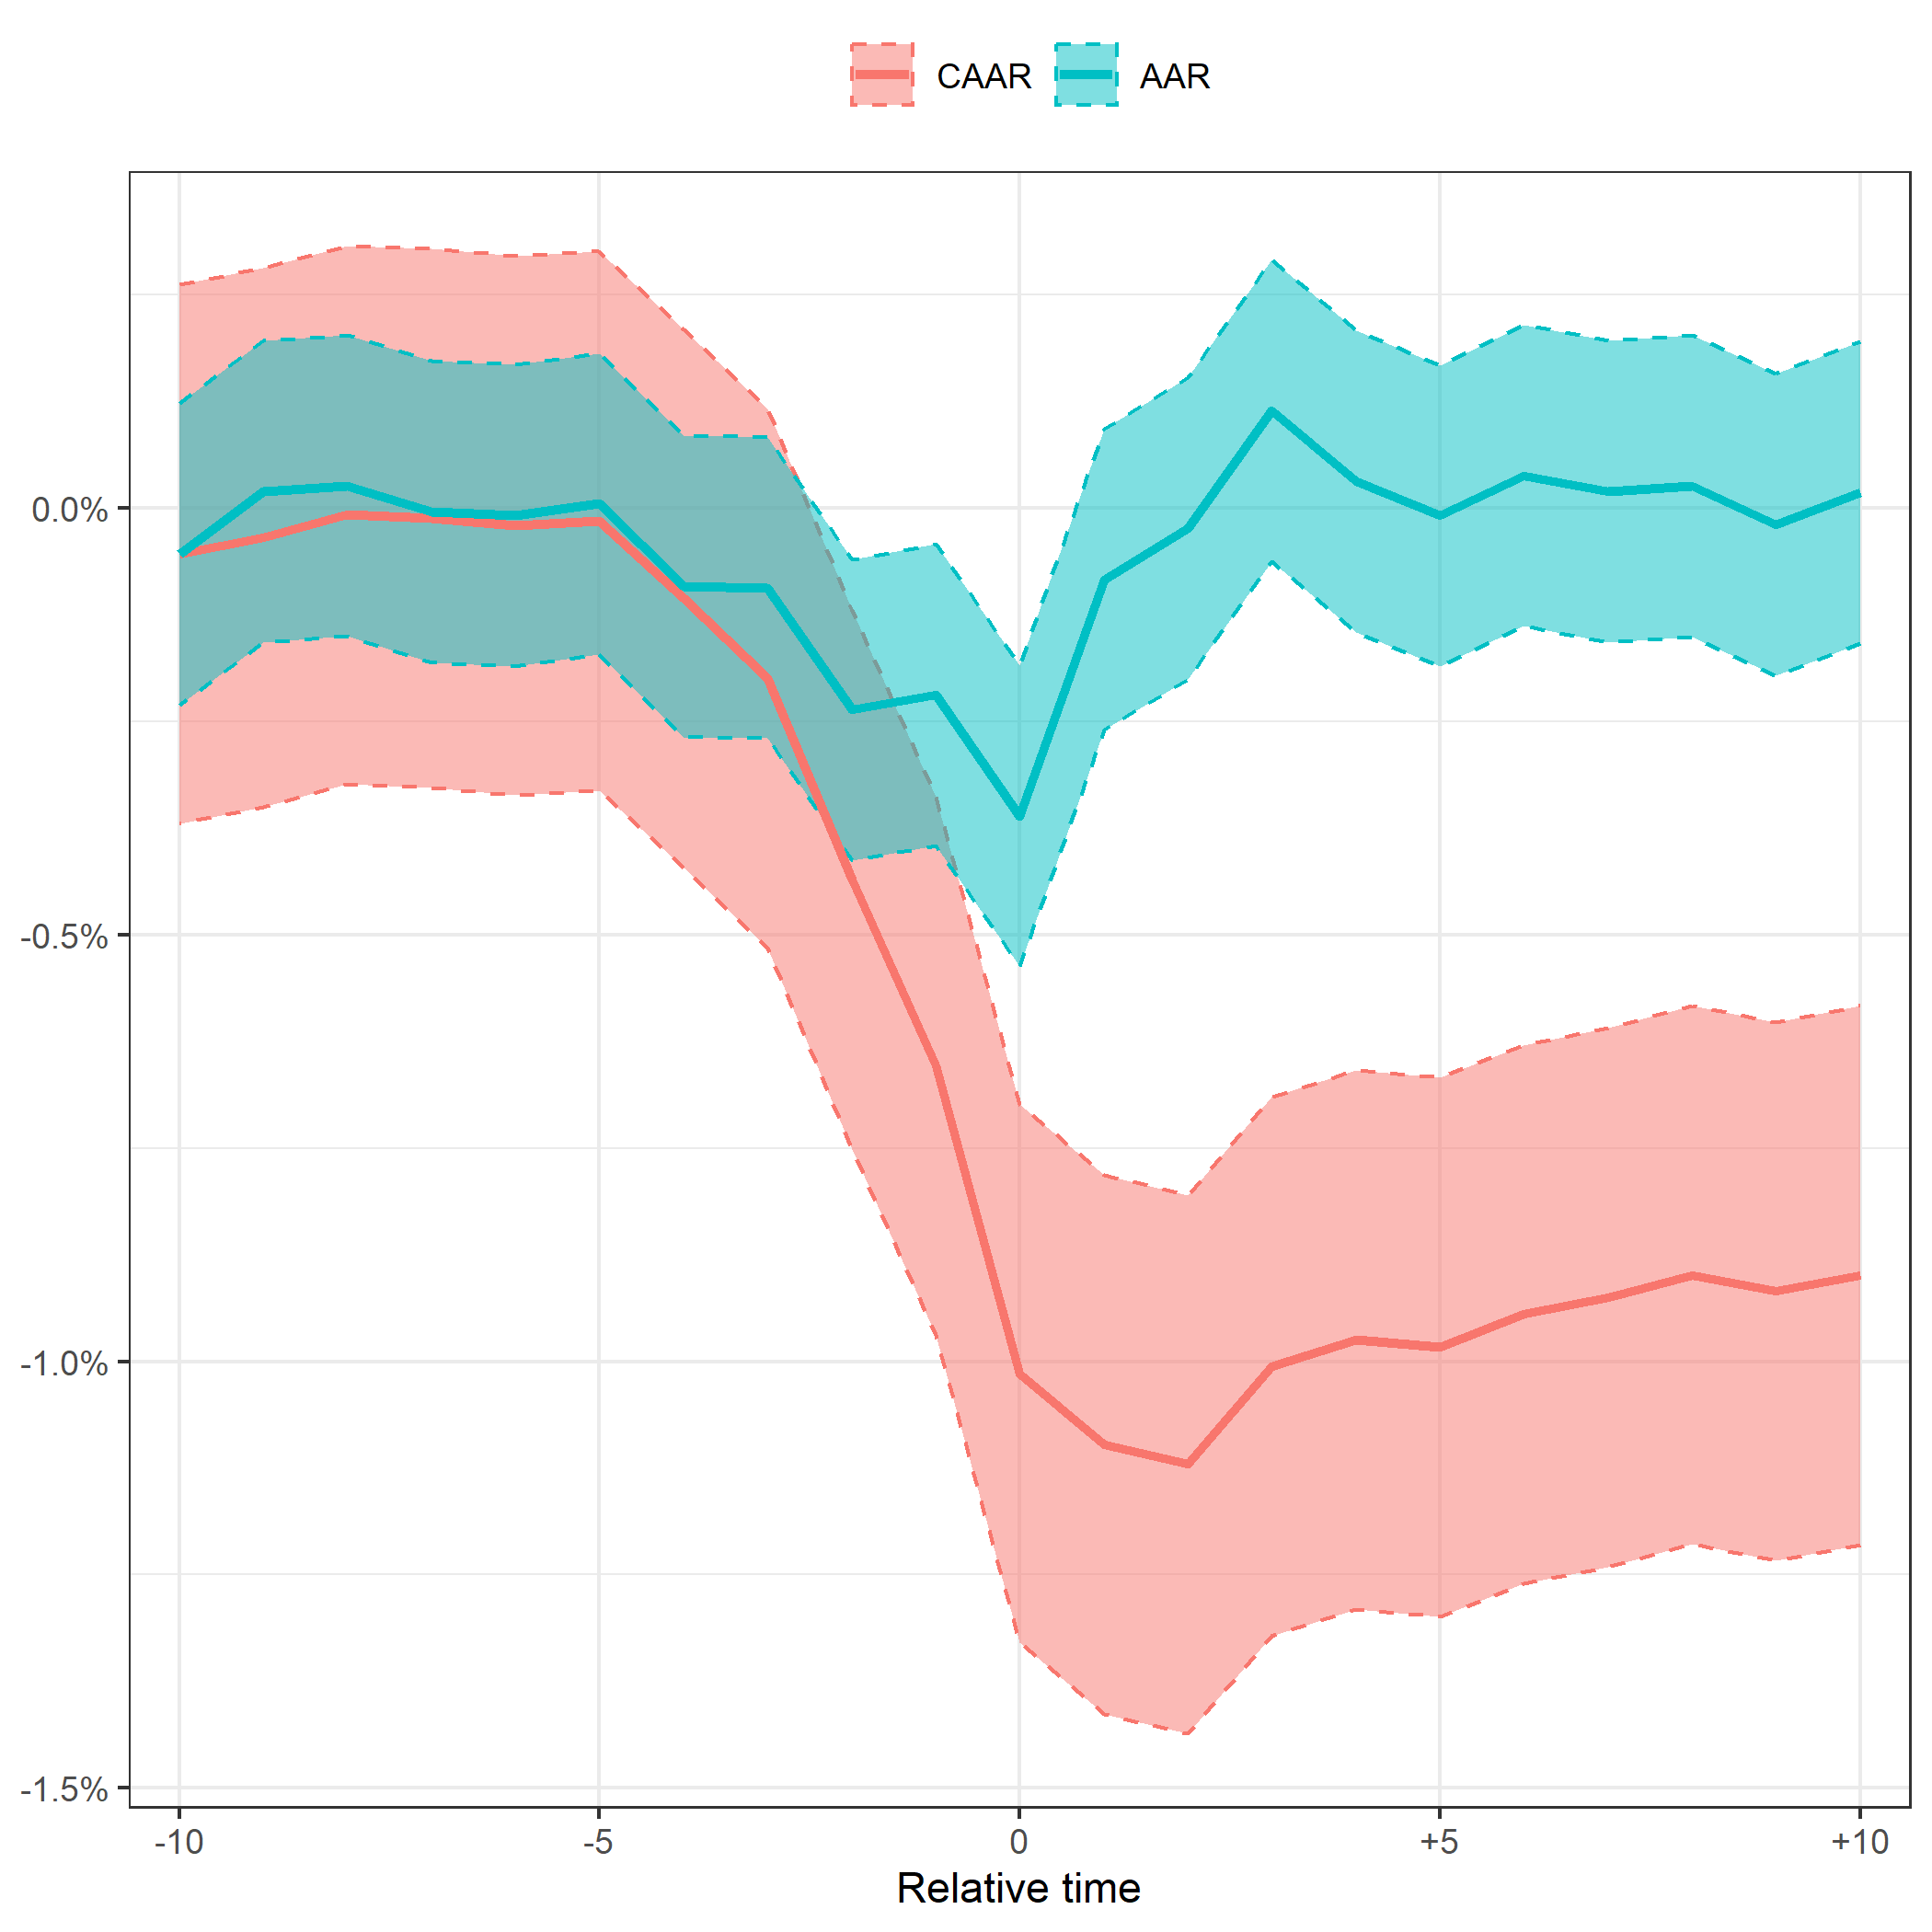
\includegraphics[scale=0.6]{Projekt/1.Figures analysis/ST_negative_all_CI.png}
     \caption*{\footnotesize The figure illustrates the average abnormal return (AAR) and cumulative AAR (CAAR) around the event date (t = 0) of negative news. The lines (left axis) represent the average and the ribbons represent the 95th confidence intervals. The bars (right axis) represent the amount of events on a given day relative to t = 0. 1618 observations }
    \label{fig:ST_neg_news}
\end{figure} 

 
The bars in the background offer insights into the extent of media attention in the days around a spike in news. For example, at $t = -1$ the average firm is mentioned in nearly 50\% less articles as the amount of the $t = 0$ day. The bars increase along with the CAAR declining in the days from $t=-7$, which imply a relation between attention towards negative news and pessimistic investor behavior even before the event date. 

The selection method for negative events was proposed to gather cases of severe negative abnormal returns. These results are an initial indication of the relation between negative news and investor reactions. 

Investigating the abnormal returns associated with news specific to the individual SDGs can potentially deepen the understanding of which themes within corporate sustainability that investors place most emphasis with. Splitting the data into 17 groups impose a natural restriction on the amount of observations of each group, which is followed by statistical uncertainty in this case. For example, SDG 4 and 9 encounter only 16 and 83 observations, respectively. The CAAR at $t=10$ per SDG are illustrated in the appendix in figure \ref{fig:ST_neg_bar_all}. With a low amount of observations the CAAR becomes highly insignificant, as indicated by the confidence intervals. To counter the issue I categorize the SDGs into five groups known officially as the Five Pillars of SDG, which consist of People, Prosperity, Planet, Peace, and Partnership\footnote{The groups consist of the following SDGs: People (1,2,3,4,5), Prosperity (7,8,9,10,11), Planet (6,12,13,14,15), Peace (16), Partnership (17)}. The analysis changes focus from the individual SDGs to broader themes within sustainability, which, regardless, allows to adequately test the hypotheses.

\begin{figure} [H]
    \centering
    \caption{SDG 5 pillars: negative news}
    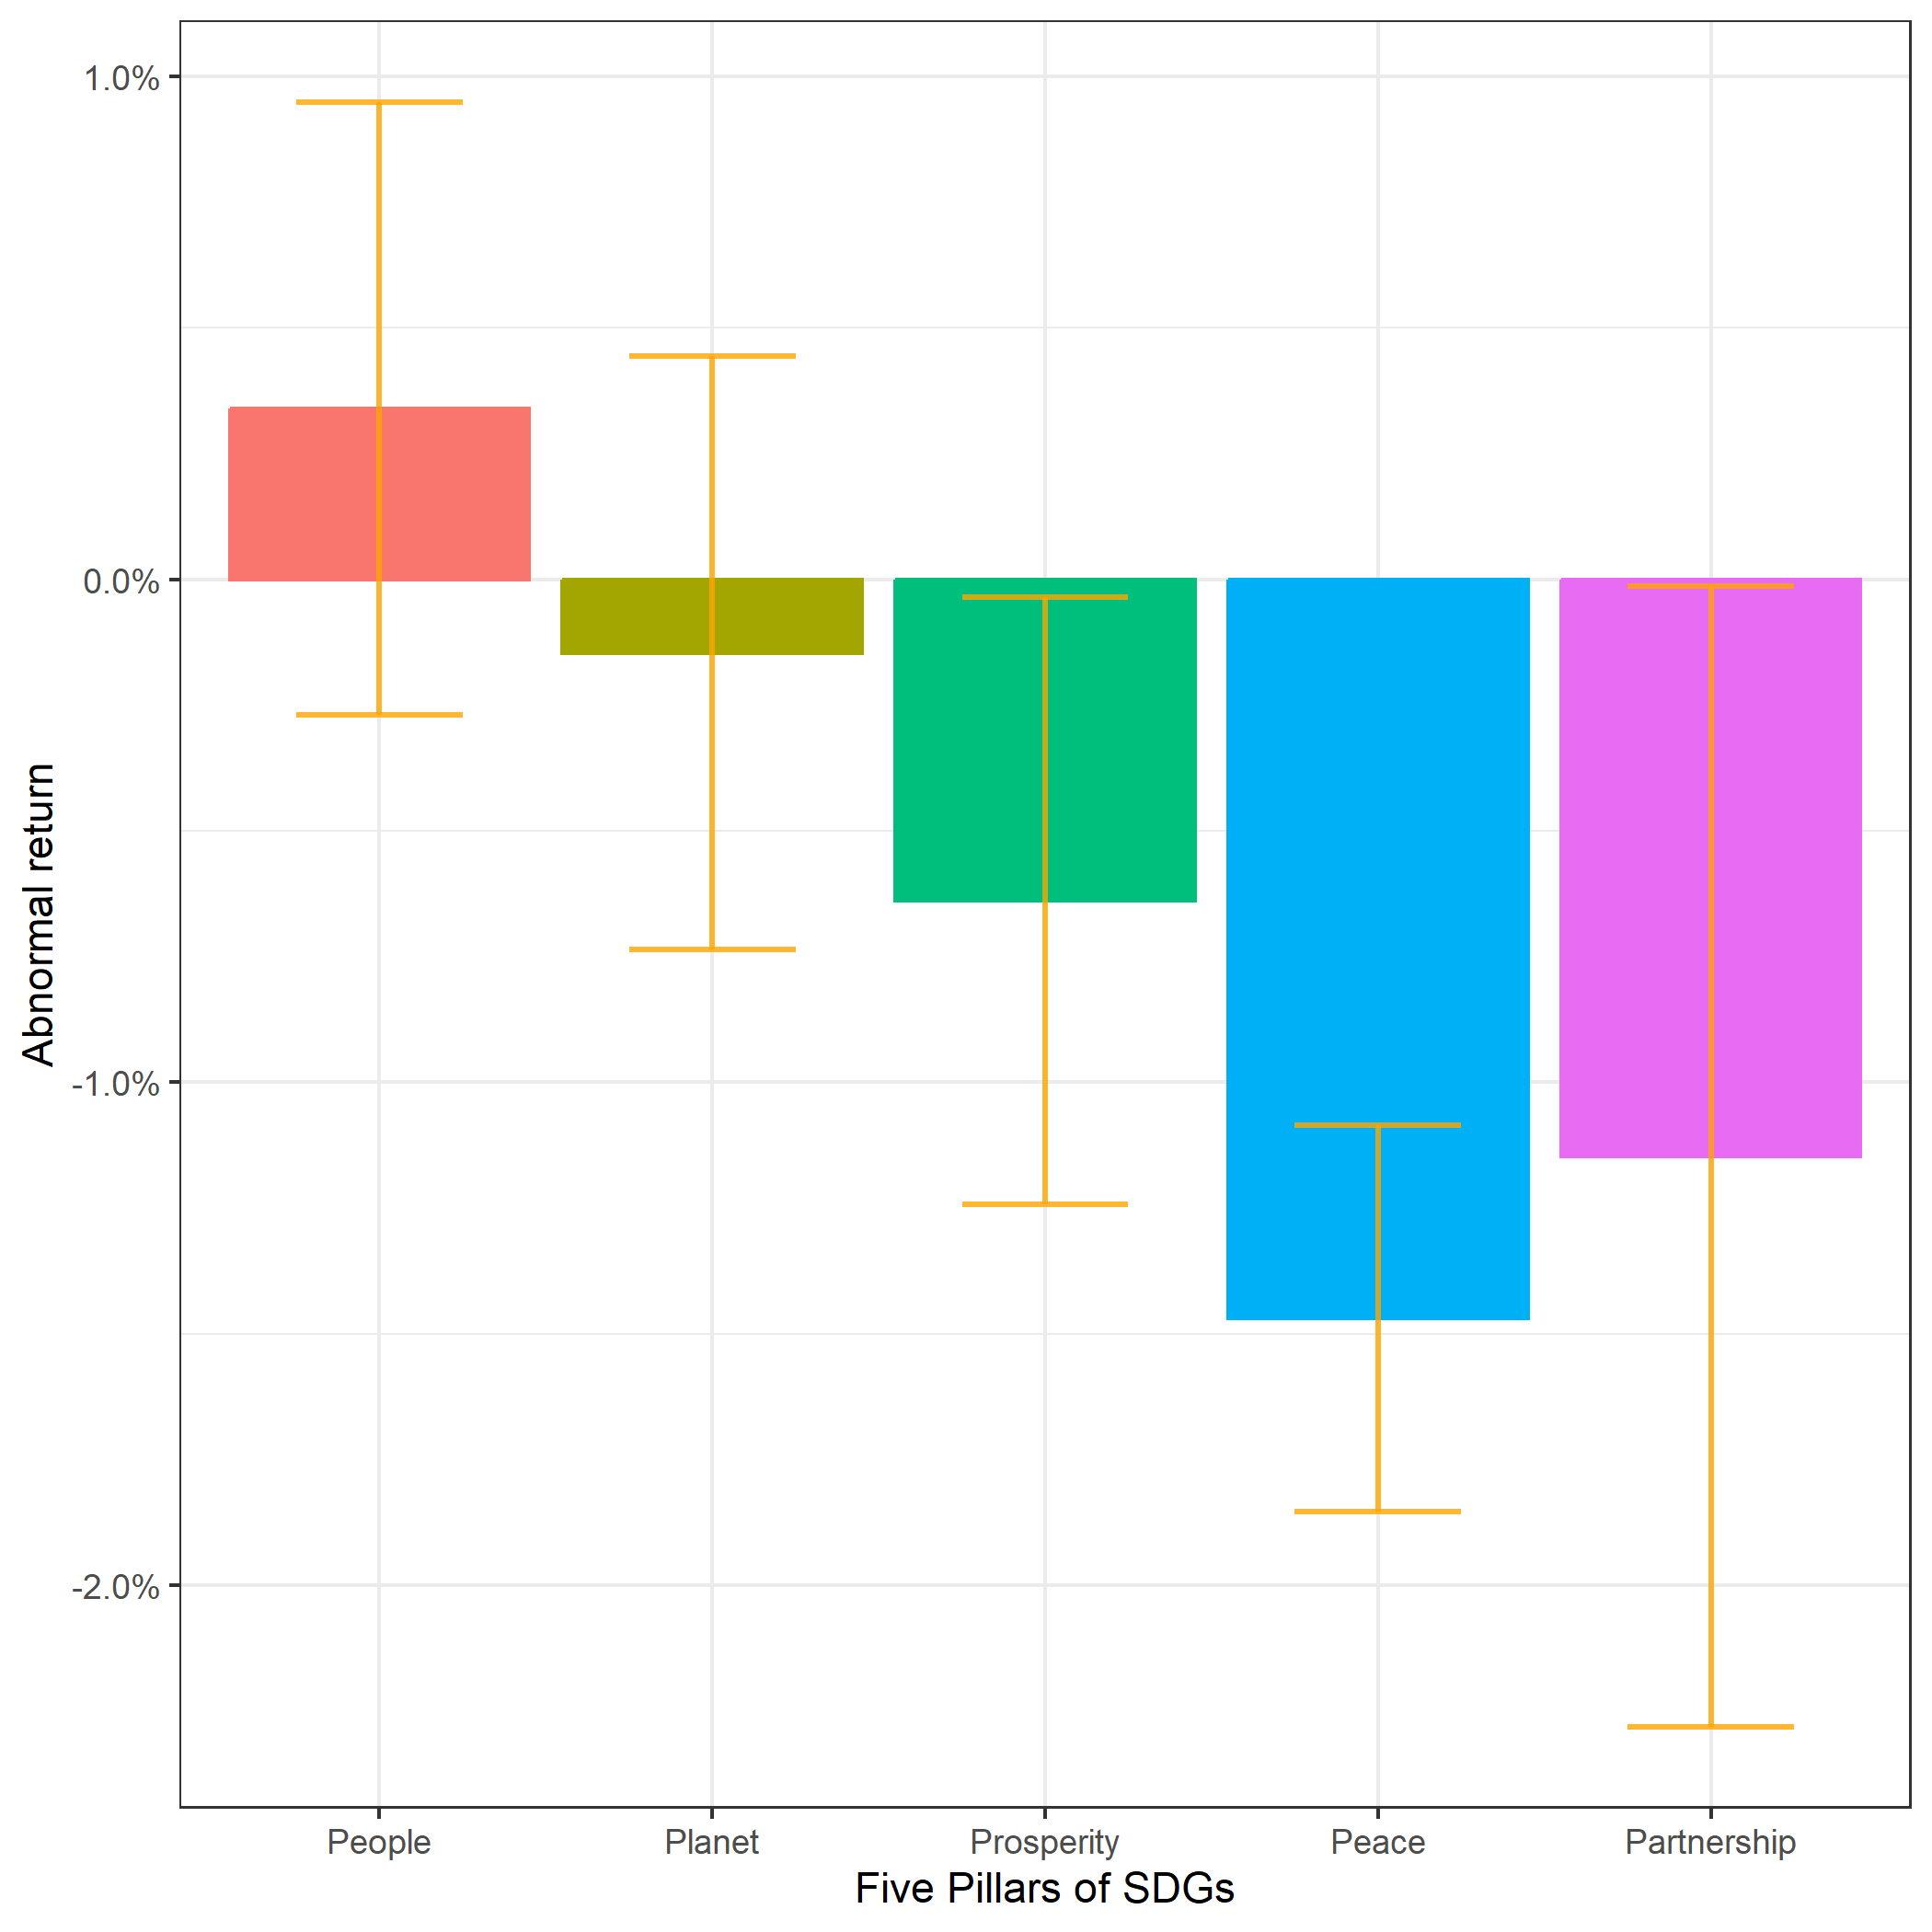
\includegraphics[scale=0.6]{Projekt/1.Figures analysis/ST_negative_sdg_bar_groups_0.png}
    \caption*{\footnotesize The figure illustrates the CAAR on $t = 10$ (the full period) from negative news. The error bars represent the 95\% confidence intervals of the CAAR.}
    \label{fig:ST_neg_bar}
\end{figure}


Figure \ref{fig:ST_neg_bar} illustrate CAAR over the full event window from negative news related to the Five Pillars of SDGs, and indicates that all groups but People are associated with negative abnormal returns. Moreover Prosperity, Peace, and Partnership are associated with significantly negative CAAR of -0.6\%, -1.5\%, and -1.1\%, respectively.       

To assess whether the degree of sustainability of firms are determinants of how abnormal returns perform after encountering news, I estimate the model with a partition on company ESG risk ratings. Figure \ref{fig:ST_neg_ESG} employs the same setup as figure \ref{fig:ST_neg_news} and displays the CAAR of event firms with a partition on ESG risk profiles. As a measure of risk, "Low" represent that a firm has a low risk of encountering complications in relation to ESG affairs.

\begin{figure} [H]
    \centering
    \caption{Negative news: CAAR split on ESG rating}
    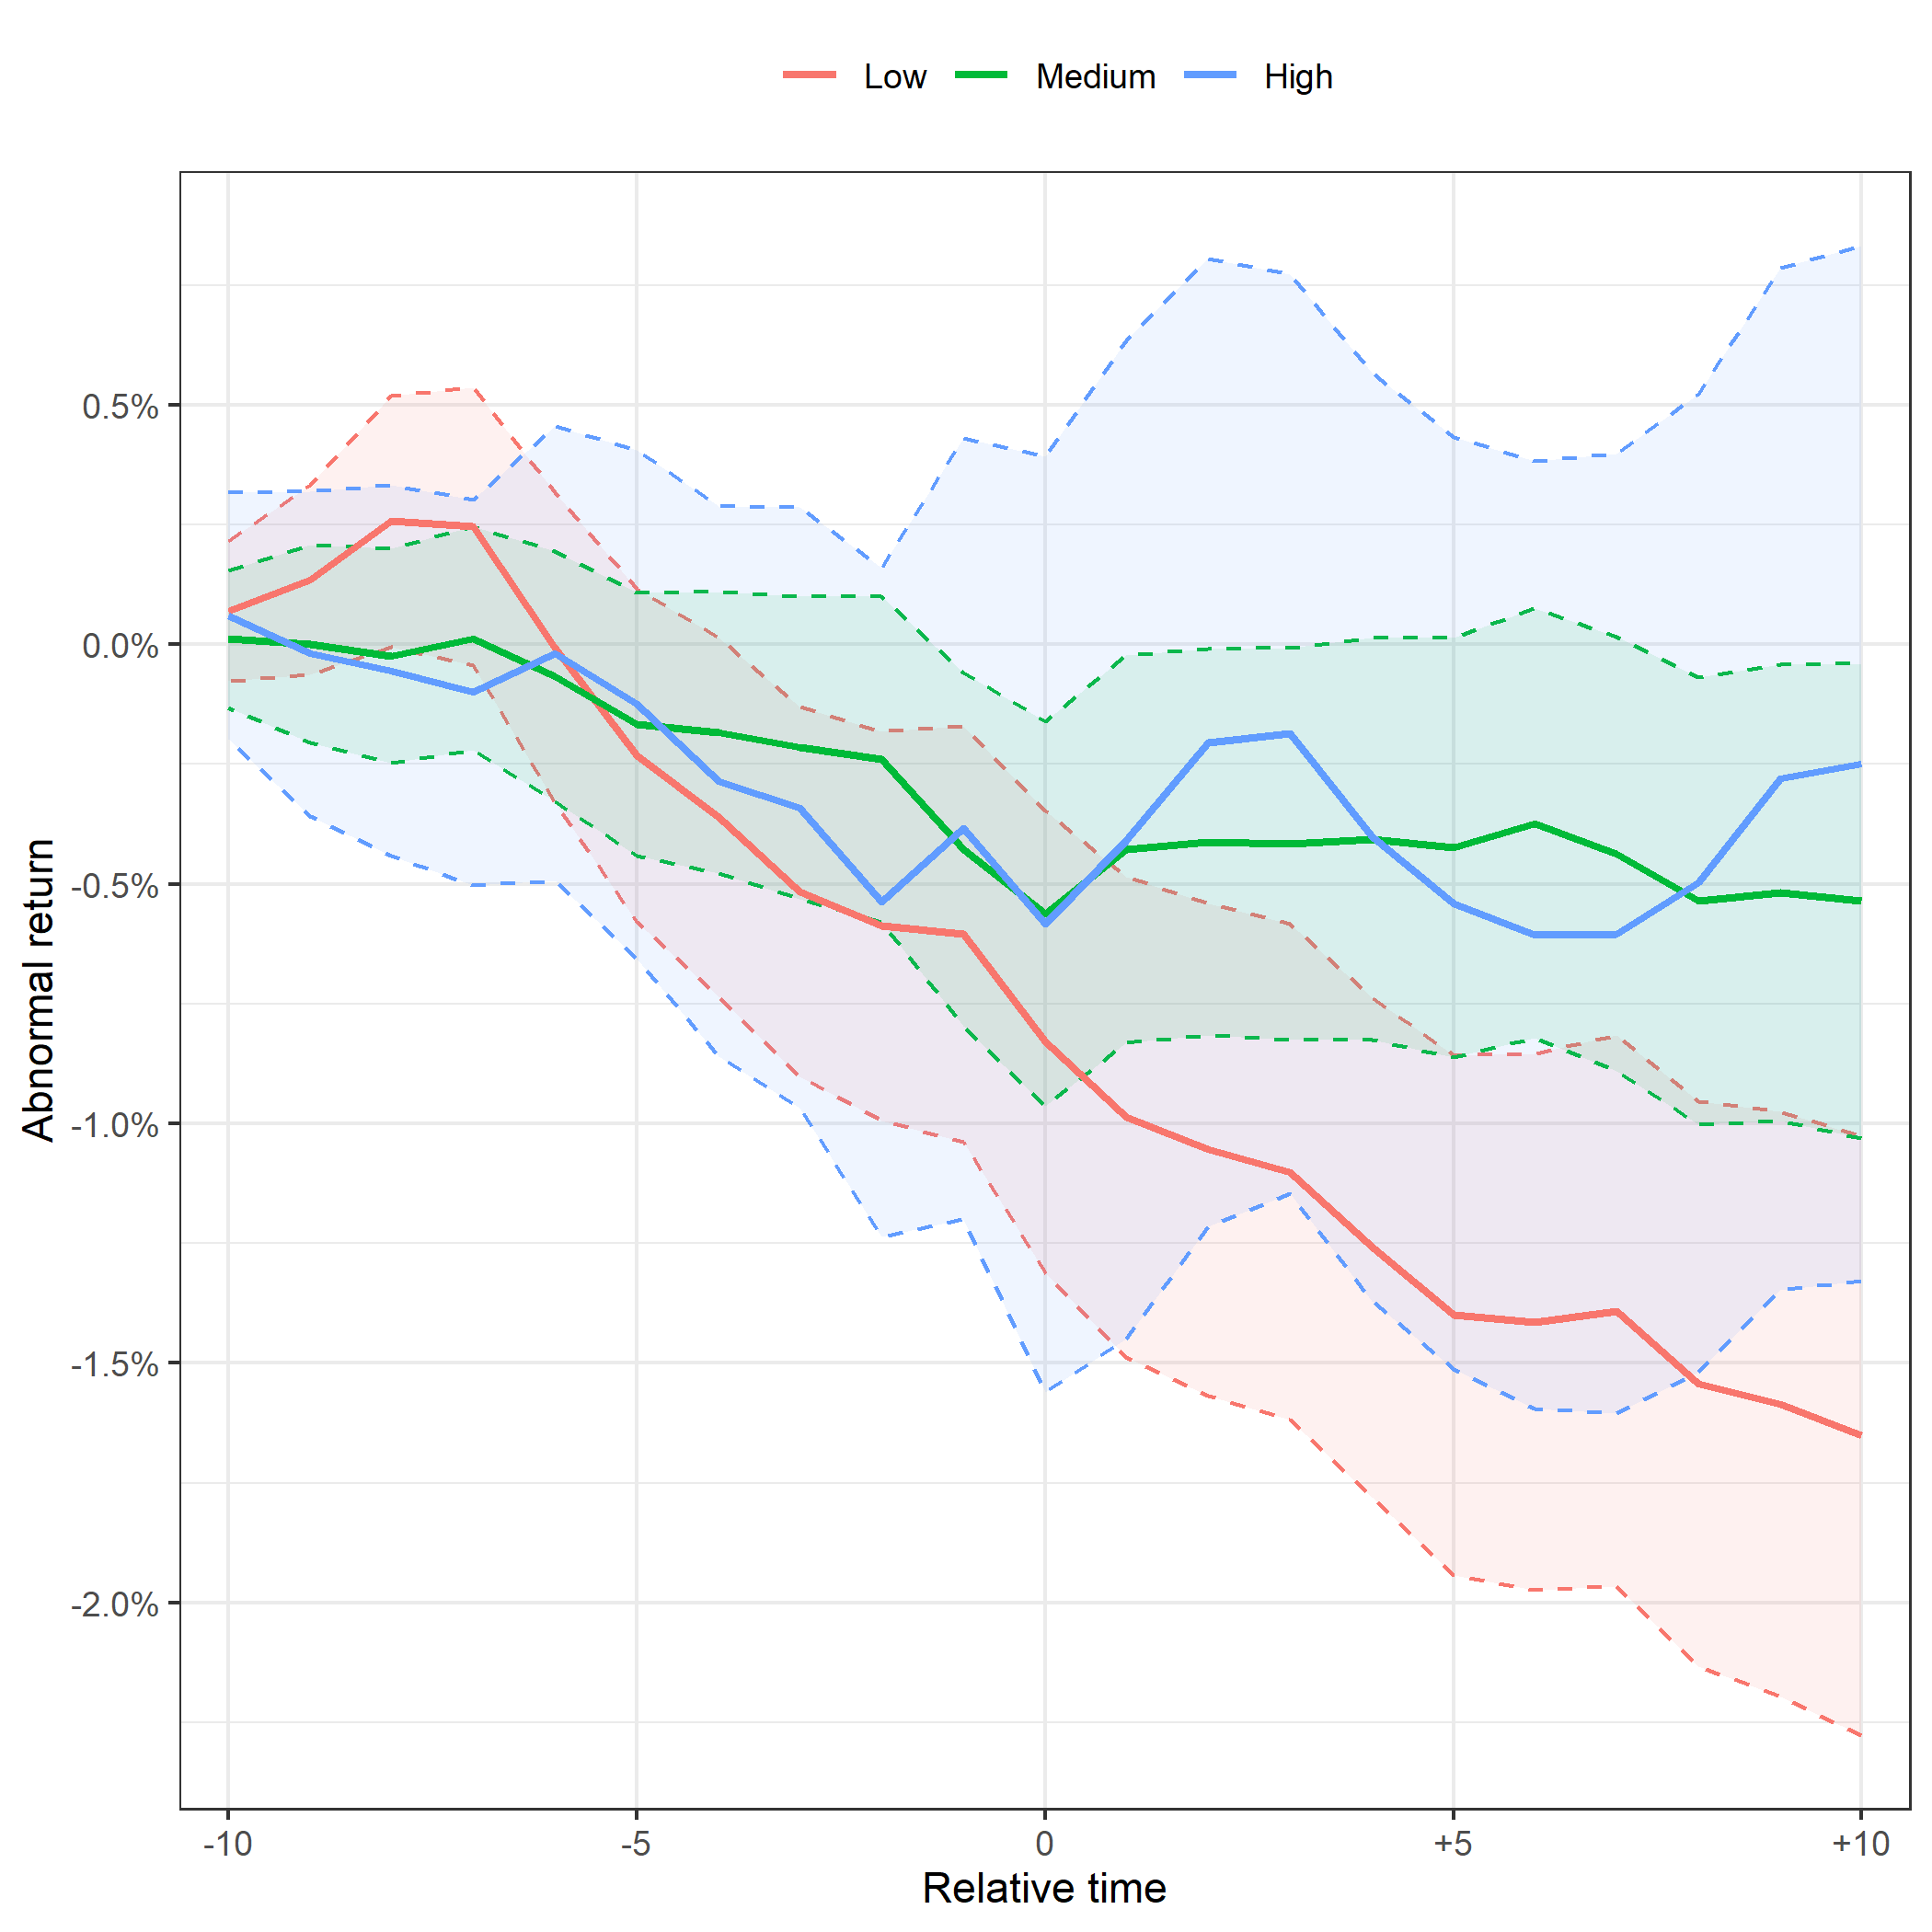
\includegraphics[scale=0.6]{Projekt/1.Figures analysis/ST_negative_ESG.png}
     \caption*{\footnotesize The figure illustrates the CAAR around the event date of negative news. The lines represent low, medium and high ESG risk of the firms in the sample. The ribbons represent the 95th confidence intervals. The categories low, medium, and high have, respectively, 504, 811, and 289 observed events in the sample. }
    \label{fig:ST_neg_ESG}
\end{figure} 


The CAAR of the three groups show dissimilar patters, indicating that the general results of negative abnormal results from figure \ref{fig:ST_neg_news} doesn't apply to all risk types. Nonetheless, firms with low and medium risk profiles both develop significant negative abnormal returns up of to -1.68\% and -0.50\%, respectively. The groups are barely statistically different from one another, however the distinction in mean values do imply a discrepancy in investor reactions. As the group of high risk companies consists of only 289 observed events, the confidence intervals become wide with a mean around -0.25\%, and no significant relation can be determined. 



\subsubsection{Positive news}

According to figure \ref{fig:ST_pos_news}, investors react promptly to positive events, as abnormal returns are present on the event day, while the remaining days of the window are not associated with a significant reaction from shareholders. The CAAR revolves around 0\% as well with a slight top on the event date. Although insignificant, a slightly positive reaction is present, however the effect reverts to zero throughout the next five days.     

\begin{figure} [H] 
    \centering
    \caption{Short term positive news: AAR and CAAR}
    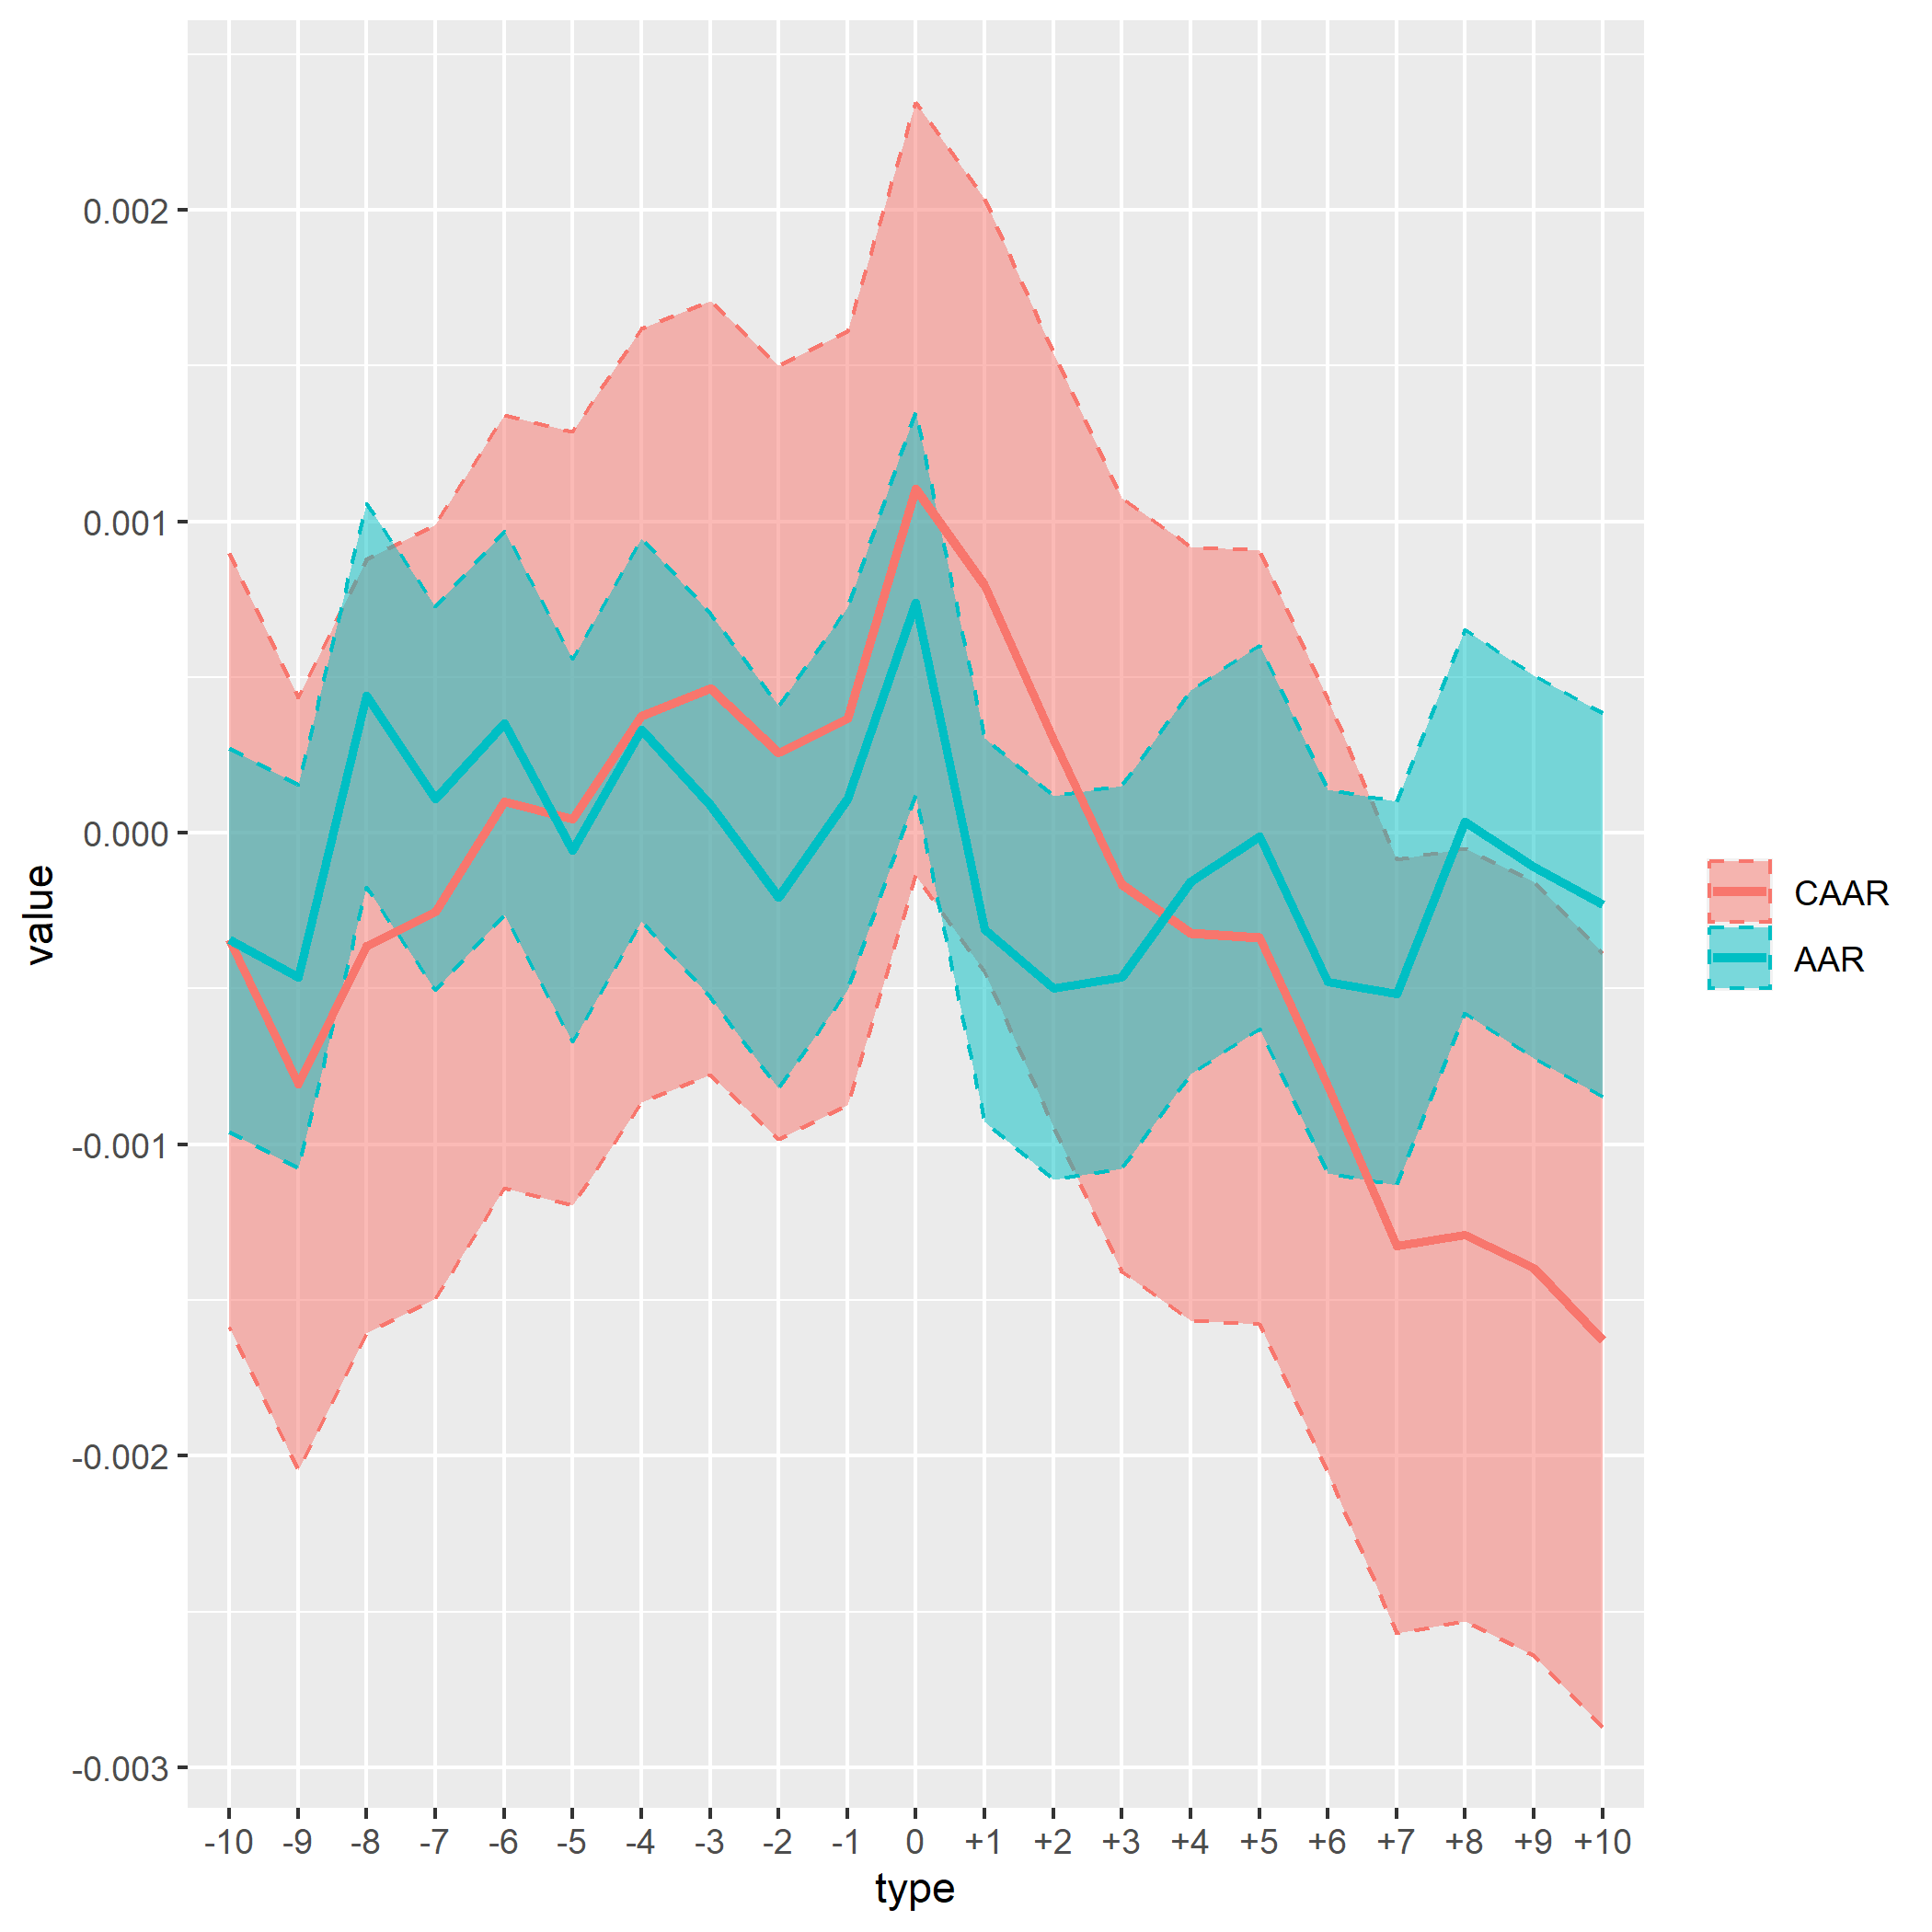
\includegraphics[scale=0.6]{Projekt/1.Figures analysis/ST_positive_all_CI.png}
    \caption*{\footnotesize The figure illustrates the average abnormal return (AAR) and cumulative AAR (CAAR) around the event date (t = 0) of positive news. The lines (left axis) represent the average and the ribbons represent the 95th confidence intervals. The bars (right axis) represent the amount of events on a given day relative to t = 0. 10420  observations}
    \label{fig:ST_pos_news}
\end{figure}

The tendencies are further emphasized by the insignificance of the abnormal returns regarding the Five Pillars of SDGs. In contrast to the case of negative events, where a potential issue involved insufficient observations, the underlying uncertainty emerge from the seemingly random shareholder reaction to positive events, as indicated by the aggregate overview in figure \ref{fig:ST_pos_bar}. People, Peace, and Partnership present negative abnormal returns, while Planet and Prosperity are positive. However, none of them are significant at a 5\% level. Only SDG 7, that deals with clean energy, display significantly abnormal returns as per figure \ref{fig:ST_pos_bar_all} in the appendix. 

\begin{figure} [H]
    \centering
    \caption{SDG 5 pillars: positive news}
    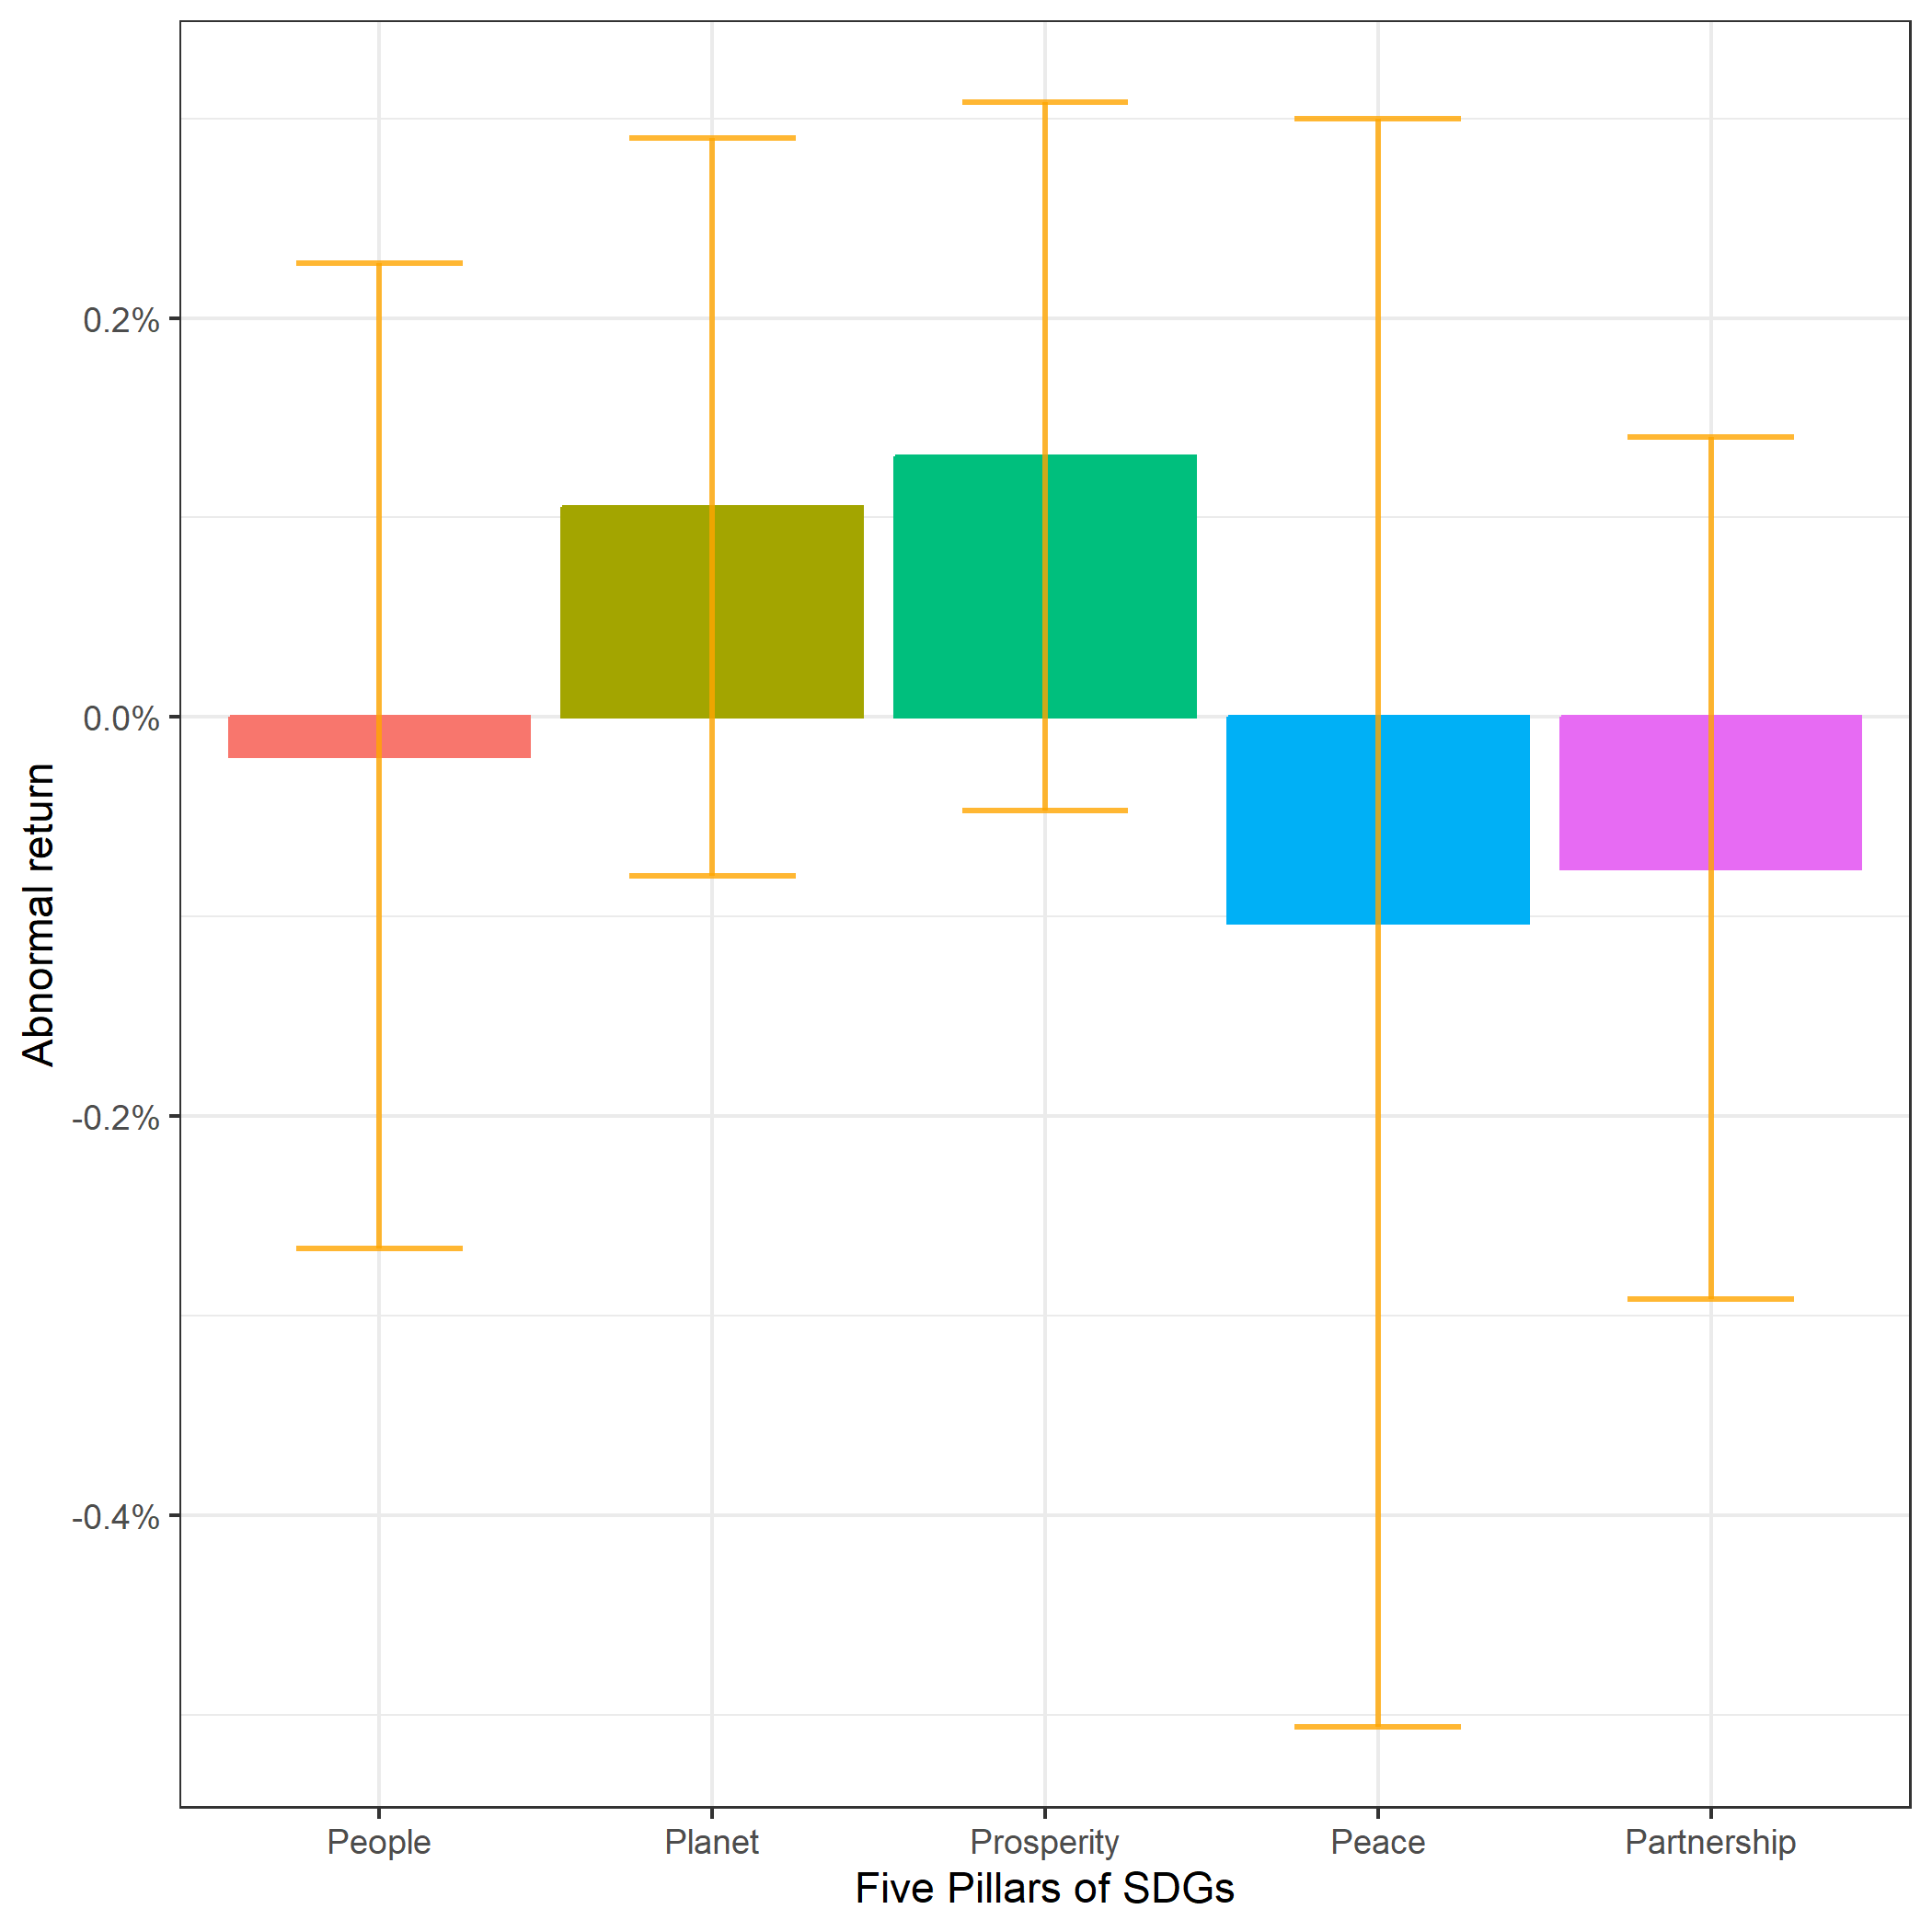
\includegraphics[scale=0.6]{Projekt/1.Figures analysis/ST_positive_sdg_bar_groups_0.png}
    \caption*{\footnotesize The figure illustrates the CAAR on $t = 10$ (full period) from positive news. The error bars represent the 95\% confidence intervals of the CAAR.}
    \label{fig:ST_pos_bar}
\end{figure}

 
Average results do not justify the full narrative as an evident difference between firms with a low and medium ESG risk profile is illustrated in figure \ref{fig:ST_pos_ESG}. With significantly negative CAAR of -0.25\% over the window, shareholders allegedly react pessimistic if low ESG risk-firms are involved in positive interactions with SDGs. High ESG risk-firms experience negative abnormal returns of the around -0.5\%, although the average comes with high uncertainty. In contrary, firms with a medium risk rating enjoy a significant, positive CAAR at $0.5\%$ over the full window. 

\begin{figure} [H]
    \centering
    \caption{Positive news: CAAR split on ESG rating}
    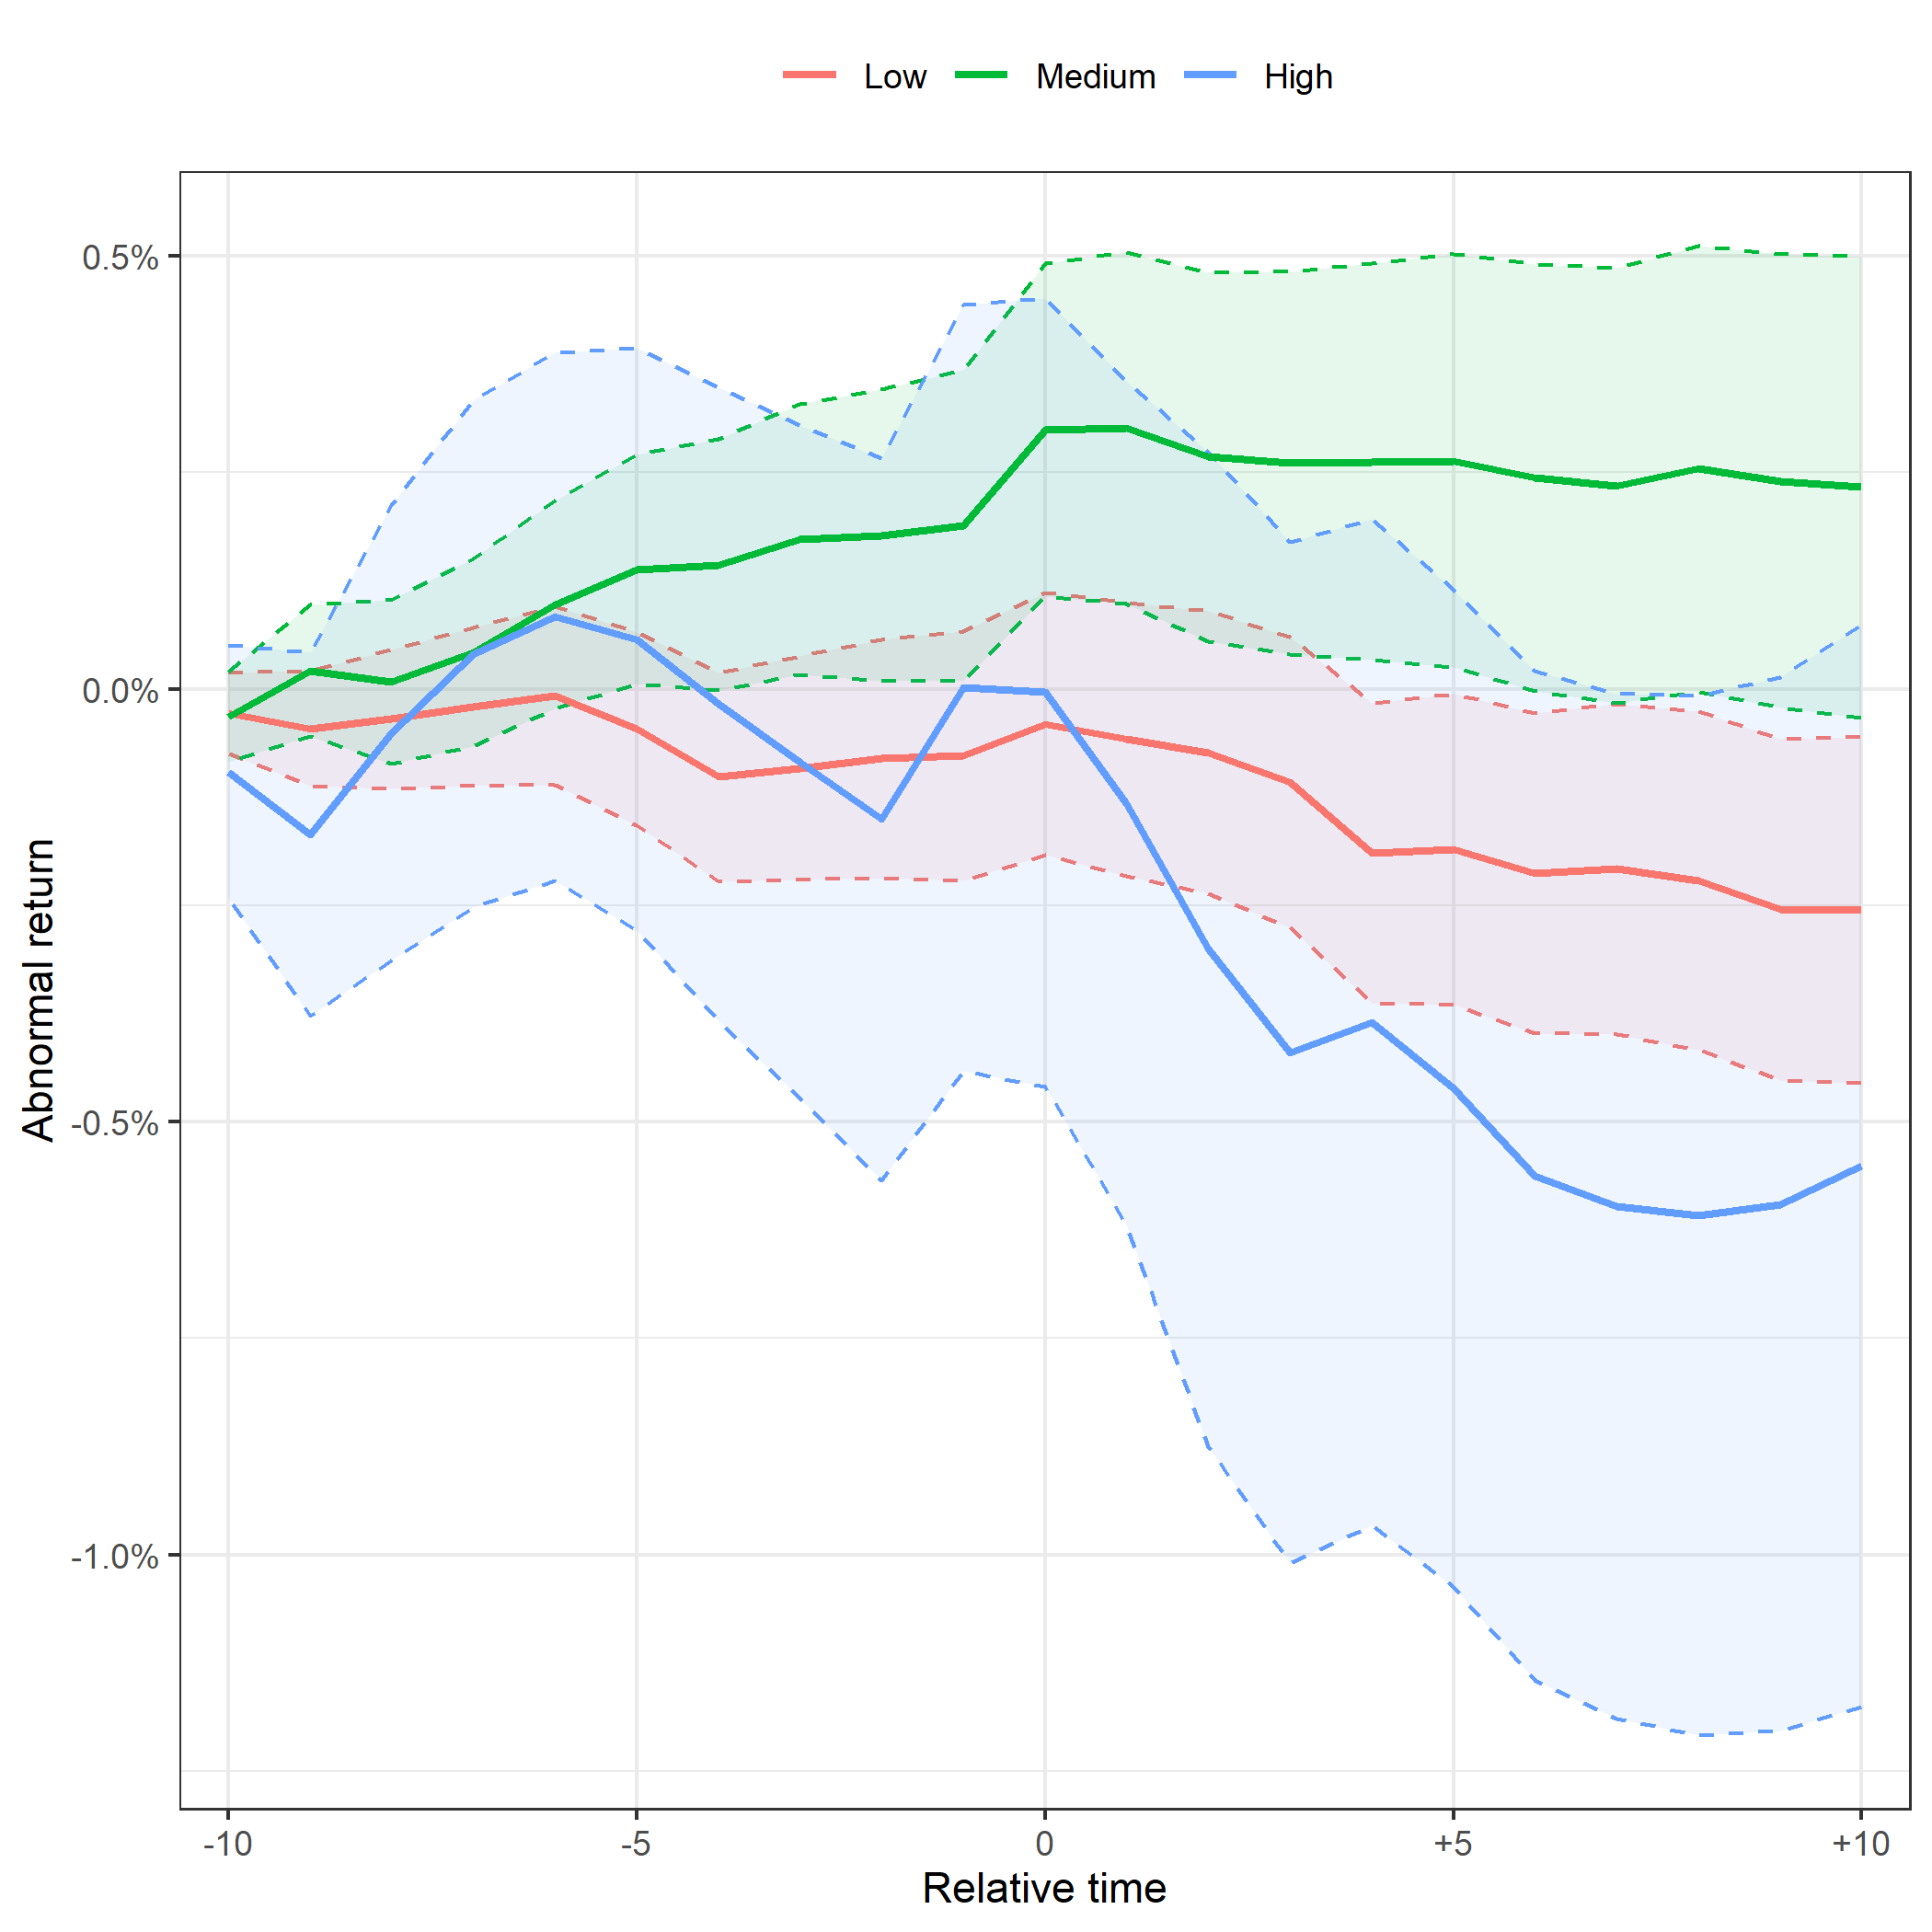
\includegraphics[scale=0.6]{Projekt/1.Figures analysis/ST_positive_ESG.png}
     \caption*{\footnotesize The figure illustrates the CAAR around the event date of positive news. The lines represent low, medium and high ESG risk of the firms in the sample. The ribbons represent the 95th confidence intervals. The categories low, medium, and high have, respectively, 4989, 4760, and 627 observed events in the sample.  }
    \label{fig:ST_pos_ESG}
\end{figure} 

Generally, the short term empirical evidence demonstrate a non-verifiable relation between abnormal returns and positive events, apart from an instant reaction on the event date.  Partitioning firms with regard to their ESG risk rating indicates that firms with medium risk are rewarded for positive news while low and high are sold off. In contrary, negative events showed a significant negative reaction on broad news and from various SDG-themes, and from medium and low risk companies.   

\subsection{Long term abnormal returns: The Calendar Time Portfolio} \label{sec: long_term_portfolio}

In contrast to the short term methodology, where all returns from events are averaged to a single event day, the long term portfolios are rebalanced each month and includes all firms, that have experienced an event within the T = 1/4/8/12 preceding months. The performance of portfolio returns are evaluated in accordance with the Calendar Time Portfolio approach, and by applying White heteroskedastic-robust standard errors. Moreover, any evidence of autocorrelation in the significant models's residuals has been rejected by a Breusch-Godfrey test of first-order. Full regression statistics including coefficient estimates, r-squared, and standard errors are available in Appendix X. The factor models do generally have high power in explaining the excess return risk exposure, with a r-square coefficient between 73\% to 98\% throughout the various portfolios. The portfolios that hold the least amount of firms on average generally has the lowest r-squared, which is a result of increased idiosyncratic variance with less observations. The inspection will not divide events into SDG themes, since the monthly amount of firms in the various portfolios would decrease to an extent where no intuition can be drawn from the results.  

\subsubsection{Negative news}

The abnormal returns from the individual portfolios are reflected through the intercept (alpha) from the Fama-French regressions in table \ref{tab: FF5_neg_ESG} along with the corresponding t-value. The table present an overall column containing the alpha from a portfolio of all firms that have experienced a negative event, and three columns representing firms split on ESG risk rating. Above each horizontal line, the "$T = x$" express the portfolio holding period after an event has occurred. 

Overall, negative events generate negative alphas for across holding periods, which indicates that the event selection methodology works as intended. The alphas are  significantly negative at -0.84\% at a $1\%$ level and -0.36\% at $5\%$ with holding periods of $T = 1$ and $T = 4$ months. Holding periods larger than four months are closer to zero and insignificant, which is in support of market efficiency on a long horizon. An implication of the strategy is that portfolios with longer holding periods will accordingly include more firms in each rebalancing, which ultimately will drive the portfolio return closer to the market return.  

\setlength{\tabcolsep}{15pt}
\begin{table}[H]
\small
\centering
\caption{Fama-French five-factor model alpha from negative news split on ESG risk} 
\begin{tabular}{llllllc}
\hline \hline \\ 
 &     & Overall &    Low  &  Medium  &  High &  \\    \cline{3-6} 
& &  \multicolumn{3}{c}{ T = 1} & \\ \cline{2-6}
& Alpha (\%)    & -0.84^{***} & -0.64^{**}  & -0.61  & -2.21 &  \\ 
& t-value   & -3.13 & -1.88 & -1.35  & -1.43 &  \\
& &  \multicolumn{3}{c}{ T = 4} & \\ \cline{2-6}
& Alpha (\%)   & -0.36^{**} & -0.23  & -0.33  &  -0.84 & \\
& t-value &   -2.29 & -1.06 & -1.28  & -1.23 & \\
& &  \multicolumn{3}{c}{ T = 8} & \\ \cline{2-6}
& Alpha (\%)    & -0.15 & -0.01   & -0.28  & -0.27 &  \\
& t-value &   -1.21 & -0.08  & -1.35 & -0.51 &  \\
& &  \multicolumn{3}{c}{ T = 12} & \\ \cline{2-6}
& Alpha (\%)    & -0.08 & -0.09  & -0.19  & -0.25 &  \\
& t-value &    -0.86 & -0.62  & -1.23 & -0.48 &  \\
\hline \hline
 \multicolumn{7}{l}{ \footnotesize $^* \; p\; <\; 0.1$, $ ^{**} \; p\; <\; 0.05$, $ ^{***} \; p\; <\; 0.01$  } \\
 \multicolumn{7}{p{12cm}}{ \footnotesize Alpha is the WLS-regression intercept (in \%) of the Fama-French 5-factor model, displayed along with the corresponding White heteroskedasticity-robust t-value. N is the average amount of firms included in the portfolio each month, and T is the portfolio holding period. The threshold for event firms to be included in the portfolio is either 1,2 or 3 "SD" (standard deviations) larger than the mean.} \\ 
 \hline
\end{tabular}
\label{tab: FF5_neg_ESG}
\end{table}

Across all subsets, the relation between negative news and returns are most severe within 1-4 months after an event has occurred. 

With a partition on ESG-risk, all alphas are negative, which confirm the initial inference. Risk characteristics of low and medium types generate alphas of approximate even magnitude at $-0.64\%$ and $-0.61\%$, respectively, with the latter being significant at 5\%. The portfolios with high ESG risk and holding periods of one and four months generates considerably larger alphas of $-2.3\%$ and $-0.84\%$.  

The monthly rebalancing contains only a few constituents as the sample of high-risk firms is small. Hence, the portfolio is exposed to idiosyncrasies, which compromise the ability of the factor models to explaining the returns through the included risk factors. Consequently, this implicates that the r-squared of regressions become very low at 0.4 and 0.53 as more of the variation ends up in the error terms. 

In general, all ESG risk types are capable of generating negative alphas. However, only firms with low ESG risk generate a significant output on average. The outcomes are more severe and with higher significance when applying shorter holding periods.   


\subsubsection{Positive news}

The impact from positive news on financial performance in the long run is illustrated in table \ref{tab: FF5_pos}. The table applies the same format as table \ref{tab: FF5_neg_ESG}. Positive events have no significant impact on returns over any of the portfolio constructions. Nevertheless, the long run effect is predominantly negative, which appears in contrast to the short term relation. Without partitioning on ESG risk, the performance is most negative when applying a brief holding period of $T=1$ with an alpha of of -0.26\%.   
Such results are indicative of a pessimistic short-to-medium term investor reaction to general positive news. However, as the alphas are insignificant in all instances, the general conclusion is that there is no relation between positive news and stock returns.  


\setlength{\tabcolsep}{15pt}
\begin{table}[H]
\small
\centering
\caption{FF-5 model alpha from positive news split on ESG risk} 
\begin{tabular}{ccccccc}
\hline \hline \\  
 &     & Overall  &    Low  &  Medium  &  High  &  \\ \cline{3-6} 
& & \multicolumn{4}{c}{ T = 1} & \\ \cline{2-6}
& Alpha (\%)  & -0.26 & -0.04  & -0.41  & -0.59 &  \\
& t-value & -1.03 & -0.12 & -1.47  & -0.47 & \\
& &  \multicolumn{4}{c}{ T = 4} & \\ \cline{2-6}
& Alpha (\%)  & -0.04 & -0.22  & -0.18  &  0.90 & \\
& t-value & -0.26 & -1.15 & -0.91  & 1.15 & \\
& &  \multicolumn{4}{c}{ T = 8} & \\ \cline{2-6}
& Alpha (\%)  & 0.01 & -0.23   & 0.03  & 1.06 &  \\
& t-value & 0.05 & 1.64  & 0.26 & 1.65 & \\
&  &  \multicolumn{4}{c}{ T = 12} & \\ \cline{2-6}
& Alpha (\%)  & 0.05 & -0.14  & 0.02  & $0.97^{*}$ &  \\
& t-value & 0.76 & -1.11  & 0.19 & 1.72 & \\
\hline \hline
 \multicolumn{7}{l}{ \footnotesize $^* \; p\; <\; 0.1$, $ ^{**} \; p\; <\; 0.05$, $ ^{***} \; p\; <\; 0.01$  } \\
 \multicolumn{7}{p{12cm}}{ \footnotesize Alpha is the WLS-regression intercept (in \%) of the Fama-French 5-factor model, displayed along with the corresponding White heteroskedasticity-robust t-values. T is the portfolio holding period. The threshold for event firms to be included in the portfolio is 1 standard deviation from the mean.}  \\ 
\end{tabular}
\label{tab: FF5_pos_ESG}
\end{table}

Applying holding periods longer than $T=1$ generates exclusively alphas close to zero, which resembles a well-diversified portfolio return close to the market portfolio, which is an expected result if positive news are recognized as irrelevant. 

With a value of -0.04\% the alpha is practically zero for the low ESG risk portfolio, while it increases to -0.41\% for medium risk, with none of the new estimates being significant. On the contrary, firms with high ESG risk seems to be rewarded with high alphas for positive events on horizons longer than four month. With T = 1 the abnormal returns are negative - on par with the short term results. However, the issue with small portfolio sizes does also apply for positive events.   

